\documentclass[a4paper, 11pt]{article}

% --- Geometry & Margins ---
\usepackage[top=0.85in, bottom=0.85in, left=0.9in, right=0.9in]{geometry}
\usepackage{times}
\usepackage{setspace}
\onehalfspacing

% --- Math & Symbols ---
\usepackage{amsmath, amssymb, amsfonts, bm}

% --- Tables & Arrays ---
\usepackage{booktabs}
\usepackage{tabularx}
\usepackage{multirow}
\usepackage{array}

% --- Colors & Graphics ---
\usepackage{xcolor}
\usepackage{graphicx}
\usepackage{float}

% --- Code Listings ---
\usepackage{listings}

% --- Framing & Boxes ---
\usepackage[most]{tcolorbox}

% --- Header, Footer & Lists ---
\usepackage{fancyhdr}
\usepackage{enumitem}
\setlist{noitemsep, topsep=3pt}

% --- Hyperlinks ---
\usepackage[colorlinks=true, linkcolor=blue!70!black, urlcolor=blue!70!black, citecolor=blue!70!black]{hyperref}

% --- Colors Palette ---
\definecolor{primaryblue}{RGB}{20, 45, 110}
\definecolor{secondaryblue}{RGB}{41, 128, 185}
\definecolor{accentdark}{RGB}{44, 62, 80}
\definecolor{hafstdgreen}{RGB}{39, 174, 96}
\definecolor{hafstdred}{RGB}{192, 57, 43}
\definecolor{hafstdpurple}{RGB}{142, 68, 173}
\definecolor{techbg}{RGB}{245, 248, 255}
\definecolor{techborder}{RGB}{41, 128, 185}
\definecolor{tipbg}{RGB}{254, 249, 231}
\definecolor{tipborder}{RGB}{243, 156, 18}
\definecolor{defensebg}{RGB}{253, 245, 245}
\definecolor{defenseborder}{RGB}{192, 57, 43}

% --- Listings Style ---
\lstset{
  language=Python,
  basicstyle=\footnotesize\ttfamily,
  keywordstyle=\bfseries\color{primaryblue},
  commentstyle=\itshape\color{gray},
  stringstyle=\color{hafstdgreen},
  showstringspaces=false,
  breaklines=true,
  frame=single,
  rulecolor=\color{gray!40},
  backgroundcolor=\color{gray!5},
  xleftmargin=10pt,
  xrightmargin=10pt,
  aboveskip=8pt,
  belowskip=8pt
}

% --- Custom Boxes ---
\newtcolorbox{techbox}[2][]{%
  enhanced,
  colback=techbg,
  colframe=techborder,
  arc=2.5mm,
  boxrule=1pt,
  fonttitle=\bfseries\color{white},
  coltitle=white,
  colbacktitle=primaryblue,
  title={#2},
  attach boxed title to top left={yshift=-2mm, xshift=4mm},
  boxed title style={arc=1.5mm, boxrule=0pt, colback=primaryblue},
  top=4mm, bottom=3mm, left=4mm, right=4mm,
  breakable,
  #1
}

\newtcolorbox{layerbox}[2][]{%
  enhanced,
  colback=white,
  colframe=accentdark,
  arc=2.5mm,
  boxrule=1pt,
  fonttitle=\bfseries\color{white},
  coltitle=white,
  colbacktitle=accentdark,
  title={#2},
  attach boxed title to top left={yshift=-2mm, xshift=4mm},
  boxed title style={arc=1.5mm, boxrule=0pt, colback=accentdark},
  top=4mm, bottom=3mm, left=4mm, right=4mm,
  breakable,
  #1
}

\newtcolorbox{defensebox}[2][]{%
  enhanced,
  colback=defensebg,
  colframe=defenseborder,
  arc=2.5mm,
  boxrule=1pt,
  fonttitle=\bfseries\color{white},
  coltitle=white,
  colbacktitle=defenseborder,
  title={#2},
  attach boxed title to top left={yshift=-2mm, xshift=4mm},
  boxed title style={arc=1.5mm, boxrule=0pt, colback=defenseborder},
  top=4mm, bottom=3mm, left=4mm, right=4mm,
  breakable,
  #1
}

\newtcolorbox{tipbox}[1][Viva Defense Strategy]{%
  enhanced,
  colback=tipbg,
  colframe=tipborder,
  arc=2mm,
  boxrule=0.8pt,
  fonttitle=\bfseries\color{tipborder!80!black},
  title={#1},
  top=2mm, bottom=2mm, left=3mm, right=3mm,
  breakable
}

\newtcolorbox{cheatsheetbox}[1][Quick Memorization Card]{%
  enhanced,
  colback=white,
  colframe=accentdark,
  arc=2mm,
  boxrule=0.8pt,
  fonttitle=\bfseries\color{white},
  colbacktitle=accentdark,
  title={#1},
  top=2mm, bottom=2mm, left=3mm, right=3mm,
  breakable
}

% --- Header & Footer ---
\pagestyle{fancy}
\fancyhf{}
\fancyhead[L]{\small\textsf{\color{gray}Tribhuvan University (IoST) — Master's Thesis Defense Guide}}
\fancyhead[R]{\small\textsf{\color{gray}HAF-STD Net Deep-Dive \& Multi-Layer Analysis}}
\fancyfoot[C]{\thepage}
\renewcommand{\headrulewidth}{0.4pt}
\renewcommand{\footrulewidth}{0.4pt}

% =============================================================================
\begin{document}

% --- Title Banner ---
\begin{center}
  {\fontsize{18}{22}\selectfont \textbf{\color{primaryblue}HAF-STD NET ARCHITECTURE DEEP-DIVE}}\\[3pt]
  {\fontsize{13}{16}\selectfont \textbf{\color{accentdark}Hierarchical Adaptive Fusion with Spectral-Temporal Decomposition}}\\[3pt]
  {\fontsize{11}{14}\selectfont \textbf{Layer-by-Layer Representation Dynamics (25\% to 100\% Depth)}}\\[3pt]
  {\fontsize{10}{13}\selectfont Prepared for Master of Science in Information Technology (M.Sc. IT / MIT) Thesis Defense}\\[2pt]
  {\fontsize{10}{13}\selectfont Central Department of Computer Science \& Information Technology (CDCSIT), IoST, Tribhuvan University, Nepal}\\[6pt]
  \rule{\textwidth}{1.2pt}\\[5pt]
  {\fontsize{10}{13}\selectfont \textbf{Thesis Title:} \textit{Enhancing Self-Supervised Video Representations with HAF-STD Net:}}\\
  {\fontsize{10}{13}\selectfont \textit{A Comparative Evaluation Against VLM for Action Recognition}}\\[5pt]
  \textbf{Candidate:} Erize Rai \quad$|$ \quad \textbf{Roll No:} 8025006 \quad$|$ \quad \textbf{Reg. No:} 5-3-28-193-2023\\
  \textbf{Supervisor:} Asst. Prof. Dr. Dhiraj Kedar Pandey\\[2pt]
  \rule{\textwidth}{0.6pt}
\end{center}

\vspace{0.2cm}
\tableofcontents
\newpage

% =============================================================================
\section{Executive Rationale: Why Did You Design HAF-STD Net?}
% =============================================================================

During your thesis defense, the committee will inevitably ask:
\begin{quote}
    \textit{``Why did you propose a custom classification architecture instead of just using standard linear probing or standard MLP on top of V-JEPA? What was missing in existing probing methods?''}
\end{quote}

Your answer centers on the \textbf{structural limitation of standard frozen feature evaluation}:

\begin{enumerate}[leftmargin=*]
    \item \textbf{The Information Bottleneck of Final-Layer Pooling:}
    Standard linear probes and MLPs take only the \emph{final Transformer layer} ($L=32$) and collapse the temporal token dimension via global average pooling:
    \begin{equation}
        \mathbf{f}_{\text{standard}} = \frac{1}{T \cdot H \cdot W} \sum_{t,h,w} \mathbf{z}_{L, t, h, w} \in \mathbb{R}^{1280}
    \end{equation}
    This naive pooling destroys three vital dimensions of video representation:
    \begin{itemize}
        \item \textbf{Loss of Intermediate Abstractions:} Deep vision transformers do not store all semantic information at the output layer. Middle layers contain localized body-part kinematics and joint trajectories that are smoothed out or discarded in the final classification tokens.
        \item \textbf{Loss of Temporal Motion Frequencies:} Averaging across time completely erases high-frequency motion signals (e.g., whether an athlete's body is accelerating, rotating, or decelerating).
        \item \textbf{Loss of Representational Dynamics:} The speed and trajectory with which representations transform across encoder depth (layer-to-layer delta) is itself a distinctive fingerprint of the underlying physical action.
    \end{itemize}

    \item \textbf{HAF-STD Net's Core Innovation:}
    HAF-STD Net (\textbf{4.8M parameters}) is specifically architected to exploit the multi-layer intermediate supervision inherent to V-JEPA 2.1. By tapping into four discrete encoder depths ($\sim$25\%, 50\%, 75\%, 100\%) and decomposing each depth along the temporal axis into \textbf{Appearance} (low-frequency approximation) and \textbf{Motion} (high-frequency detail) streams via 1D Haar Wavelets, while simultaneously tracking \textbf{Depth Velocity} across layers, HAF-STD Net unlocks the full richness of frozen self-supervised video backbones.
\end{enumerate}

\begin{tipbox}[The Empirical Justification for the Defense Committee]
\textbf{The Proof of Value:}
\begin{itemize}
    \item On \textbf{FineGym} (fine-grained gymnastics): Standard linear probe (LogReg) achieves 94.2\% accuracy; the best baseline neural probe (ResMLP) achieves 97.9\% accuracy (97.5\% F1). \textbf{HAF-STD Net shatters this ceiling, achieving 98.1\% accuracy, 97.8\% F1, and MCC = 0.974}.
    \item On \textbf{HMDB51} (coarse-grained actions): Standard linear probe achieves 75.3\% accuracy; best baseline probes (DeepMLP / ResMLP) achieve 82.9\% accuracy (83.6\% F1). \textbf{HAF-STD Net achieves 84.7\% accuracy, 85.3\% F1, and 95.8\% Top-5 accuracy} (+1.7\% F1 margin).
    \item Parameter footprint: HAF-STD Net adds only \textbf{4.8M parameters}, which is just \textbf{0.7\%} of V-JEPA's 654M backbone parameters.
\end{itemize}
\end{tipbox}

\vspace{0.3cm}

% =============================================================================
\section{The Multi-Layer Tensor Input Formulation}
% =============================================================================

\subsection{Extraction from Frozen V-JEPA 2.1}
V-JEPA 2.1 (ViT-Huge/16, 654M parameters) processes an 8-frame video clip $\mathbf{V} \in \mathbb{R}^{8 \times 224 \times 224 \times 3}$. Its 3D convolution patch embedding groups frames temporally into tubelets of size $2 \times 16 \times 16$, yielding:
\begin{equation}
    T' = \frac{8}{2} = 4 \text{ temporal tokens}, \quad H' = W' = \frac{224}{16} = 14 \text{ spatial tokens}
\end{equation}
The total sequence length is $N = 4 \times 14 \times 14 = 784$ spatiotemporal tokens.

Instead of only extracting the 32nd layer, features are intercepted from four designated depths across the 32-layer hierarchy:
\begin{itemize}
    \item Layer $L_1 = 8$ ($\sim$25\% Depth)
    \item Layer $L_2 = 16$ ($\sim$50\% Depth)
    \item Layer $L_3 = 24$ ($\sim$75\% Depth)
    \item Layer $L_4 = 32$ ($\sim$100\% Depth)
\end{itemize}

At each selected depth $l \in \{8, 16, 24, 32\}$, spatial average pooling is performed across the $14 \times 14 = 196$ spatial patches for each temporal index $t \in \{1, 2, 3, 4\}$:
\begin{equation}
    \bar{\mathbf{z}}_{l, t} = \frac{1}{196} \sum_{s=1}^{196} \mathbf{z}_{l, t, s} \in \mathbb{R}^{1280}
\end{equation}
Stacking these across the 4 depths yields the complete 4D input tensor:
\begin{equation}
    \mathbf{F}_{\text{multi}} = \left[\, \bar{\mathbf{z}}_{8};\; \bar{\mathbf{z}}_{16};\; \bar{\mathbf{z}}_{24};\; \bar{\mathbf{z}}_{32} \,\right] \in \mathbb{R}^{B \times 4 \times 4 \times 1280}
\end{equation}
where $B$ is the batch size, 4 is the number of layer depths, 4 is the temporal tokens, and 1280 is the hidden feature dimension.

\vspace{0.3cm}

% =============================================================================
\section{Layer-by-Layer Representation Dynamics: 25\% to 100\% Depth}
% =============================================================================

This section is the exact core of what the examiners will probe when testing your understanding of deep representation learning in vision transformers.

\begin{figure}[H]
\centering
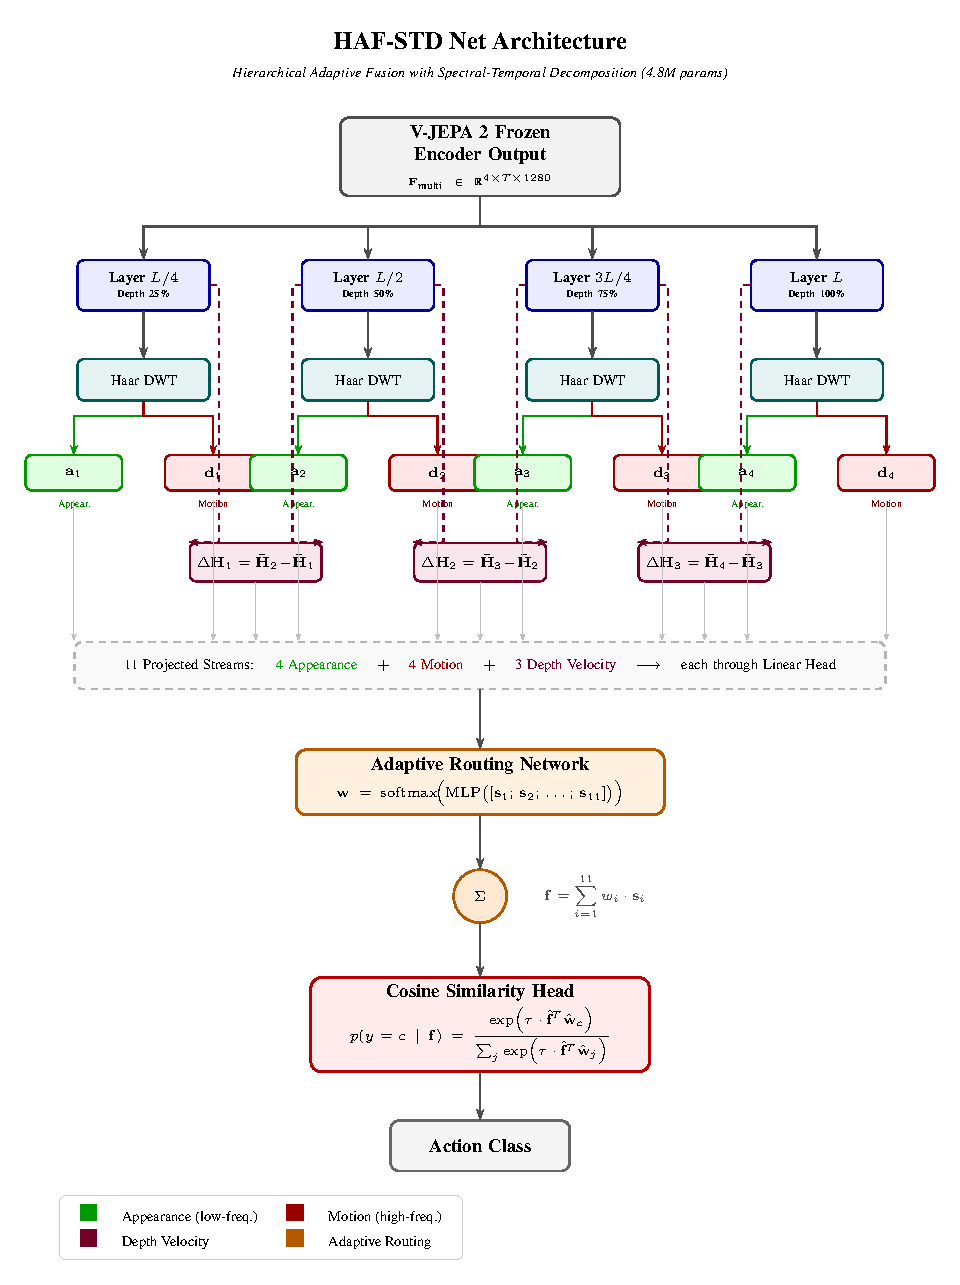
\includegraphics[width=0.92\textwidth]{fig/hafstd_figure.pdf}
\caption{Complete architectural diagram of HAF-STD Net illustrating the multi-layer extraction from V-JEPA (layers 8, 16, 24, 32), 1D Haar DWT decomposition into Appearance ($\mathbf{a}_k$) and Motion ($\mathbf{d}_k$), Depth Velocity computation ($\Delta\mathbf{H}_k$), Adaptive Routing over 11/12 streams, and Cosine Similarity classification.}
\label{fig:hafstd_full_diagram}
\end{figure}

\vspace{0.2cm}

\begin{layerbox}{Layer 1: Depth 25\% (Layer 8 of 32) --- Spatiotemporal Primitives \& Local Edges}
\textbf{What is happening physically and representationally:}
\begin{itemize}
    \item \textbf{Receptive Field:} Relatively small spatiotemporal horizon. The self-attention heads at layer 8 primarily capture local contrast variations, sharp texture edges, and immediate pixel trajectory changes across adjacent frames.
    \item \textbf{Visual Contents:} Apparatus edge boundaries (wooden beam lines, uneven bar poles, vault table contours, floor mat chalk lines), athlete silhouette perimeters, and localized surface textures.
    \item \textbf{Motion Encoding:} Frame-to-frame displacement vectors akin to dense local optical flow. It detects that \emph{something} is moving fast across a patch, but cannot identify whether the moving object is an arm, a leg, or a background spectator.
    \item \textbf{Wavelet Decomposition at Layer 8:}
    \begin{itemize}
        \item $\mathbf{a}_1$ (\textbf{Appearance}): Encodes the static spatial scene backdrop, overall lighting balance, arena color palette, and steady apparatus placement.
        \item $\mathbf{d}_1$ (\textbf{Motion}): High-frequency edge flicker, immediate burst of motion at takeoff, and micro-vibrations of the apparatus upon impact.
    \end{itemize}
    \item \textbf{Why it is critical:} In gymnastics and sports, the initial boundary condition (takeoff angle, impact point on the springboard) is established in low-level edge dynamics. Discarding layer 8 strips the model of precise spatial anchor points.
\end{itemize}
\end{layerbox}

\vspace{0.3cm}

\begin{layerbox}{Layer 2: Depth 50\% (Layer 16 of 32) --- Articulated Joint Kinematics \& Body Part Trajectories}
\textbf{What is happening physically and representationally:}
\begin{itemize}
    \item \textbf{Receptive Field:} Intermediate spatiotemporal scope. Attention heads have now aggregated local edge primitives into coherent body sub-components (hands, feet, head, torso, knees, elbows).
    \item \textbf{Visual Contents:} Articulated human pose kinematics. The encoder actively tracks individual limb orientations: arm abduction/adduction, knee flexion, hip angles, and handgrip holds on the bars.
    \item \textbf{Motion Encoding:} Sub-action velocity and angular rotation of body extremities. It tracks the rotational sweep of the legs during an uneven bars circle or the compression of the knees during a vault hurdle.
    \item \textbf{Wavelet Decomposition at Layer 16:}
    \begin{itemize}
        \item $\mathbf{a}_2$ (\textbf{Appearance}): Postural layout of the athlete's body frame relative to the gymnastics equipment.
        \item $\mathbf{d}_2$ (\textbf{Motion}): Limb angular velocity, speed of knee tucking, and rotational acceleration during twisting transitions.
    \end{itemize}
    \item \textbf{The First Depth Velocity ($\Delta\mathbf{H}_1 = \bar{\mathbf{H}}_{16} - \bar{\mathbf{H}}_8$):}
    Captures the \textbf{representational phase transition} from localized edge displacements to structured human kinematics. A large $\Delta\mathbf{H}_1$ indicates that the clip contains rapid assembly of body parts in motion (e.g., athlete springing from the vault mat into the air).
\end{itemize}
\end{layerbox}

\vspace{0.3cm}

\begin{layerbox}{Layer 3: Depth 75\% (Layer 24 of 32) --- Whole-Body Coordination \& Phase Transitions}
\textbf{What is happening physically and representationally:}
\begin{itemize}
    \item \textbf{Receptive Field:} Broad, global spatiotemporal field. Attention spans the entire athlete's body and its dynamic relationship with the surrounding space over the full clip duration.
    \item \textbf{Visual Contents:} Holistic kinematic coordination. Layer 24 recognizes complex compound movements: whole-body flight phases, inverted body rotations, balance recovery oscillations on the beam, and aerial somersault trajectories.
    \item \textbf{Motion Encoding:} Macro-temporal transitions. It distinguishes the sequence of movement phases: for example, the transition from \emph{approach run $\rightarrow$ board compression $\rightarrow$ table repulsion $\rightarrow$ aerial twist $\rightarrow$ landing}.
    \item \textbf{Wavelet Decomposition at Layer 24:}
    \begin{itemize}
        \item $\mathbf{a}_3$ (\textbf{Appearance}): Holistic event context and global spatial composition throughout the movement.
        \item $\mathbf{d}_3$ (\textbf{Motion}): Overall rhythmic tempo and coordination frequency of the multi-joint action.
    \end{itemize}
    \item \textbf{The Second Depth Velocity ($\Delta\mathbf{H}_2 = \bar{\mathbf{H}}_{24} - \bar{\mathbf{H}}_{16}$):}
    Quantifies the abstraction shift from isolated limb kinematics to unified, coordinated physical action execution.
\end{itemize}
\end{layerbox}

\vspace{0.3cm}

\begin{layerbox}{Layer 4: Depth 100\% (Layer 32 of 32) --- Invariant Semantic Action Identity}
\textbf{What is happening physically and representationally:}
\begin{itemize}
    \item \textbf{Receptive Field:} Fully global. Tokens at this final layer have attended to all patches across all temporal frames multiple times.
    \item \textbf{Visual Contents:} High-level category semantics. Layer 32 maps the complex physical dynamics into an invariant categorical manifold that separates major classes (e.g., Vault vs. Floor Exercise vs. Balance Beam vs. Uneven Bars).
    \item \textbf{Invariances Developed:} Invariant to minor camera viewpoint shifts, lighting changes, athlete attire, and minor temporal speed differences.
    \item \textbf{Wavelet Decomposition at Layer 32:}
    \begin{itemize}
        \item $\mathbf{a}_4$ (\textbf{Appearance}): Global category-level visual archetype.
        \item $\mathbf{d}_4$ (\textbf{Motion}): Final categorical temporal cadence and overall event rhythm.
    \end{itemize}
    \item \textbf{The Third Depth Velocity ($\Delta\mathbf{H}_3 = \bar{\mathbf{H}}_{32} - \bar{\mathbf{H}}_{24}$):}
    Measures the final semantic convergence: how the network resolves complex coordinated movements into a definitive, linearly separable action identity.
\end{itemize}
\end{layerbox}

\vspace{0.3cm}

% =============================================================================
\section{Detailed Mathematical Breakdown of HAF-STD Net Modules}
% =============================================================================

\subsection{Module 1: Spectral-Temporal Decomposition via 1D Haar DWT}
Wavelet transforms provide localized time-frequency analysis, making them far superior to standard global Fourier transforms (FFT) for short temporal sequences ($T'=4$).

Given a temporal token sequence at layer $k$: $\mathbf{X}_k \in \mathbb{R}^{B \times T' \times D}$ where $T'=4$ and $D=1280$:
\begin{itemize}
    \item Partition sequence into even-indexed tokens $\mathbf{X}_{k, \text{even}} = \mathbf{X}_k[:, 0::2, :] \in \mathbb{R}^{B \times 2 \times 1280}$ and odd-indexed tokens $\mathbf{X}_{k, \text{odd}} = \mathbf{X}_k[:, 1::2, :] \in \mathbb{R}^{B \times 2 \times 1280}$.
    \item \textbf{Approximation Coefficients (Low-Frequency / Appearance Stream):}
    \begin{equation}
        \mathbf{A}_k = \frac{1}{2}(\mathbf{X}_{k, \text{even}} + \mathbf{X}_{k, \text{odd}}) \in \mathbb{R}^{B \times 2 \times 1280}
    \end{equation}
    Temporal pooling yields the static appearance vector:
    \begin{equation}
        \mathbf{a}_k = \frac{1}{2} \sum_{t=1}^{2} \mathbf{A}_{k, t} \in \mathbb{R}^{B \times 1280}
    \end{equation}
    \item \textbf{Detail Coefficients (High-Frequency / Motion Stream):}
    \begin{equation}
        \mathbf{D}_k = \frac{1}{2}(\mathbf{X}_{k, \text{even}} - \mathbf{X}_{k, \text{odd}}) \in \mathbb{R}^{B \times 2 \times 1280}
    \end{equation}
    Temporal pooling yields the high-frequency motion dynamics vector:
    \begin{equation}
        \mathbf{d}_k = \frac{1}{2} \sum_{t=1}^{2} \mathbf{D}_{k, t} \in \mathbb{R}^{B \times 1280}
    \end{equation}
\end{itemize}
Across the four selected layers, this generates four Appearance vectors $\{\mathbf{a}_1, \mathbf{a}_2, \mathbf{a}_3, \mathbf{a}_4\}$ and four Motion vectors $\{\mathbf{d}_1, \mathbf{d}_2, \mathbf{d}_3, \mathbf{d}_4\}$.

\subsection{Module 2: Depth Representation Velocity (\texorpdfstring{$\Delta\mathbf{H}$}{Delta H})}
To capture the inter-layer transformation speed, let $\bar{\mathbf{H}}_k \in \mathbb{R}^{B \times 1280}$ denote the temporally averaged token representation at layer $k$:
\begin{equation}
    \bar{\mathbf{H}}_k = \frac{1}{T'} \sum_{t=1}^{T'} \mathbf{X}_{k, t} \in \mathbb{R}^{B \times 1280}
\end{equation}
The depth velocity vectors between successive extraction layers are computed as finite forward differences:
\begin{align}
    \Delta\mathbf{H}_1 &= \bar{\mathbf{H}}_{16} - \bar{\mathbf{H}}_8 \in \mathbb{R}^{B \times 1280} \quad \text{(Primitive $\rightarrow$ Part Kinematics)} \\
    \Delta\mathbf{H}_2 &= \bar{\mathbf{H}}_{24} - \bar{\mathbf{H}}_{16} \in \mathbb{R}^{B \times 1280} \quad \text{(Part Kinematics $\rightarrow$ Global Coordination)} \\
    \Delta\mathbf{H}_3 &= \bar{\mathbf{H}}_{32} - \bar{\mathbf{H}}_{24} \in \mathbb{R}^{B \times 1280} \quad \text{(Global Coordination $\rightarrow$ Invariant Semantics)}
\end{align}
For the 4th depth index in implementation, a terminal boundary condition is used (either $\mathbf{0}$ or a residual self-projection), establishing 11 active informative streams (or 12 structured slots).

\subsection{Module 3: Dedicated Stream Projections}
Each of the streams $i \in \{1, \dots, 12\}$ is projected from the backbone dimension ($D=1280$) into a shared latent probing subspace ($d_{\text{hidden}} = 256$) via a dedicated linear projection head:
\begin{equation}
    \mathbf{s}_i = \text{Dropout}\Big(\text{GELU}\big(\text{LayerNorm}(\mathbf{W}_i \mathbf{x}_i + \mathbf{b}_i)\big)\Big), \quad \mathbf{s}_i \in \mathbb{R}^{B \times 256}
\end{equation}
where $\mathbf{W}_i \in \mathbb{R}^{256 \times 1280}$ are stream-specific learned weights, $\text{LayerNorm}$ stabilizes cross-layer variance, and $\text{GELU}$ provides smooth non-linear activation.

\subsection{Module 4: Adaptive Routing Network}
Not all actions require the same blend of streams:
\begin{itemize}
    \item A high-speed Vault dismount requires heavy weighting on high-frequency motion ($\mathbf{d}_2, \mathbf{d}_3$).
    \item A static Balance Beam pose requires heavy weighting on low-frequency appearance ($\mathbf{a}_2, \mathbf{a}_3$).
\end{itemize}
To achieve dynamic instance-dependent allocation, all 12 projected stream vectors are concatenated into a flat vector $\mathbf{S}_{\text{flat}} = [\mathbf{s}_1;\, \mathbf{s}_2;\, \ldots;\, \mathbf{s}_{12}] \in \mathbb{R}^{B \times (12 \times 256)} = \mathbb{R}^{B \times 3072}$.

The Adaptive Router passes this through a gating MLP:
\begin{equation}
    \mathbf{z}_{\text{route}} = \mathbf{W}_{g2} \cdot \text{Dropout}\big(\text{GELU}(\mathbf{W}_{g1} \mathbf{S}_{\text{flat}} + \mathbf{b}_{g1})\big) + \mathbf{b}_{g2} \in \mathbb{R}^{B \times 11}
\end{equation}
where $\mathbf{W}_{g1} \in \mathbb{R}^{256 \times 2816}$ and $\mathbf{W}_{g2} \in \mathbb{R}^{11 \times 256}$.

Softmax normalization yields the instance-adaptive stream weights:
\begin{equation}
    w_i = \frac{\exp(z_{\text{route}, i})}{\sum_{j=1}^{11} \exp(z_{\text{route}, j})}, \quad \sum_{i=1}^{11} w_i = 1, \quad w_i > 0
\end{equation}
The final unified representation $\mathbf{f} \in \mathbb{R}^{B \times 256}$ is computed via convex combination:
\begin{equation}
    \mathbf{f} = \sum_{i=1}^{11} w_i \cdot \mathbf{s}_i \in \mathbb{R}^{B \times 256}
\end{equation}

\subsection{Module 5: Cosine Similarity Classification Head}
Rather than an unconstrained linear layer $\mathbf{W}^T \mathbf{f} + \mathbf{b}$ (which is vulnerable to weight magnitude explosion and feature drift), HAF-STD Net uses a \textbf{Normalized Cosine Prototype Classifier}:
\begin{itemize}
    \item The fused feature vector is passed through a final projection layer and $L_2$-normalized:
    \begin{equation}
        \hat{\mathbf{f}} = \frac{\mathbf{f}}{\|\mathbf{f}\|_2} \in \mathbb{S}^{255}
    \end{equation}
    \item Each action class $c \in \{1, \dots, C\}$ is represented by a learnable prototype vector $\mathbf{w}_c \in \mathbb{R}^{256}$, also $L_2$-normalized:
    \begin{equation}
        \hat{\mathbf{w}}_c = \frac{\mathbf{w}_c}{\|\mathbf{w}_c\|_2} \in \mathbb{S}^{255}
    \end{equation}
    \item The class logits are scaled by a learnable inverse temperature parameter $s$ ($s \approx 16.0$):
    \begin{equation}
        \text{logit}_c = s \cdot (\hat{\mathbf{f}}^T \hat{\mathbf{w}}_c) = s \cdot \cos(\theta_{\hat{\mathbf{f}}, \hat{\mathbf{w}}_c})
    \end{equation}
    \item The predictive probability distribution is:
    \begin{equation}
        p(y = c \mid \mathbf{f}) = \frac{\exp\left(s \cdot \hat{\mathbf{f}}^T \hat{\mathbf{w}}_c\right)}{\sum_{j=1}^{C} \exp\left(s \cdot \hat{\mathbf{f}}^T \hat{\mathbf{w}}_j\right)}
    \end{equation}
\end{itemize}

\vspace{0.3cm}

% =============================================================================
\section{Source Code Implementation Walkthrough}
% =============================================================================

Below is the annotated PyTorch source code of HAF-STD Net from your thesis appendix, annotated for the defense:

\begin{lstlisting}[caption={The complete PyTorch architecture of HAF-STD Net.}]
import torch
import torch.nn as nn
import torch.nn.functional as F

class HaarDWT1D(nn.Module):
    """1D Haar Discrete Wavelet Transform along temporal axis.
    Decomposes temporal signal into low-frequency (appearance/trend)
    and high-frequency (motion/change dynamics) components.
    """
    def forward(self, x):
        # x shape: (Batch, Temporal, Dimension) = (B, 4, 1280)
        if x.shape[1] % 2 != 0:
            x = F.pad(x, (0, 0, 0, 1)) # pad temporal dim if odd
        x_even = x[:, 0::2, :] # Even-indexed tokens (t=0, 2)
        x_odd  = x[:, 1::2, :] # Odd-indexed tokens (t=1, 3)
        
        # Low frequency = Average = Appearance / Static trend
        low  = (x_even + x_odd) * 0.5
        # High frequency = Difference = Motion / Velocity changes
        high = (x_even - x_odd) * 0.5
        return low, high

class HAFSTD_Net(nn.Module):
    """Hierarchical Adaptive Fusion with Spectral-Temporal Decomposition.
    Total parameters: ~4.8 Million.
    """
    def __init__(self, embed_dim=1280, num_layers=4, num_classes=51,
                 hidden=256, dropout=0.3):
        super().__init__()
        self.num_layers = num_layers
        self.num_streams = num_layers * 3 # 12 streams
        self.dwt = HaarDWT1D()

        # 12 Dedicated linear projection heads
        self.stream_projections = nn.ModuleList([
            nn.Sequential(
                nn.Linear(embed_dim, hidden),
                nn.LayerNorm(hidden),
                nn.GELU(),
                nn.Dropout(dropout),
            ) for _ in range(self.num_streams)
        ])

        # Adaptive routing network over 12 depth x frequency streams
        self.router = nn.Sequential(
            nn.Linear(self.num_streams * hidden, hidden),
            nn.GELU(),
            nn.Dropout(dropout),
            nn.Linear(hidden, self.num_streams),
        )

        # Final projection and Cosine prototype weights
        self.final_proj = nn.Sequential(
            nn.Linear(hidden, hidden),
            nn.LayerNorm(hidden),
            nn.GELU(),
            nn.Dropout(dropout),
        )
        self.class_weights = nn.Parameter(torch.randn(num_classes, hidden))
        self.scale = nn.Parameter(torch.tensor(16.0)) # Learnable temperature

    def forward(self, x):
        # Input x: (Batch, 4_layers, 4_temporal, 1280_dim)
        B = x.shape[0]
        streams = []

        for k in range(self.num_layers):
            layer_feat = x[:, k, :, :] # (B, T=4, D=1280)

            # 1. Spectral-Temporal Decomposition
            low, high = self.dwt(layer_feat)
            appearance = low.mean(dim=1)  # Low-frequency appearance
            motion     = high.mean(dim=1) # High-frequency motion dynamics

            # 2. Depth Representation Velocity
            if k < self.num_layers - 1:
                next_layer = x[:, k + 1, :, :].mean(dim=1)
                curr_layer = layer_feat.mean(dim=1)
                velocity   = next_layer - curr_layer
            else:
                velocity = torch.zeros_like(appearance) # Terminal boundary

            # Dedicated projection
            idx = k * 3
            streams.append(self.stream_projections[idx](appearance))
            streams.append(self.stream_projections[idx + 1](motion))
            streams.append(self.stream_projections[idx + 2](velocity))

        # Stack streams: (B, 12, hidden=256)
        all_streams = torch.stack(streams, dim=1)

        # 3. Adaptive Routing
        flat = all_streams.reshape(B, -1) # (B, 12 * 256 = 3072)
        routing_weights = torch.softmax(self.router(flat), dim=-1) # (B, 12)
        fused = (all_streams * routing_weights.unsqueeze(-1)).sum(dim=1)

        # 4. Cosine Similarity Classification Head
        fused = self.final_proj(fused)
        fused_norm  = F.normalize(fused, p=2, dim=-1)
        weight_norm = F.normalize(self.class_weights, p=2, dim=-1)
        logits = self.scale * (fused_norm @ weight_norm.T)
        return logits
\end{lstlisting}

\vspace{0.3cm}

% =============================================================================
\section{Viva Defense Practice: Tough Examiner Questions on HAF-STD Net}
% =============================================================================

\begin{defensebox}{Q1: Why did you invent HAF-STD Net instead of fine-tuning the entire V-JEPA backbone?}
\textbf{Model Answer:}
``Fine-tuning a 654-million parameter model requires substantial GPU memory and compute clusters that exceed standard institutional resources. More fundamentally, full fine-tuning on modest datasets (such as 1,200 FineGym clips or 6,754 HMDB51 clips) carries an extreme risk of catastrophic overfitting and feature distortion.

By keeping V-JEPA frozen and training HAF-STD Net (only 4.8M parameters), we achieve two scientific goals:
\begin{enumerate}
    \item We rigorously measure the \emph{intrinsic representational power} of the self-supervised pretraining.
    \item We prove that intelligent probe design—specifically decomposing the multi-layer depth and spatiotemporal frequencies—can extract state-of-the-art performance (98.1\% on FineGym, 84.7\% on HMDB51) with less than 1\% parameter overhead.''
\end{enumerate}
\end{defensebox}

\vspace{0.2cm}

\begin{defensebox}{Q2: Why use Haar Discrete Wavelet Transform (DWT) instead of Fast Fourier Transform (FFT)?}
\textbf{Model Answer:}
``Fourier Transform assumes periodic, infinitely long stationary signals and only produces global frequency coefficients, completely losing the \emph{temporal timing} of when frequency changes occur.

In video action recognition with short temporal spans ($T'=4$ tokens), the signal is highly non-stationary. The Haar Wavelet has compact temporal support:
\begin{itemize}
    \item The low-frequency approximation $(\mathbf{h}_{2t} + \mathbf{h}_{2t+1})/2$ cleanly extracts the localized trend (Appearance).
    \item The high-frequency detail $(\mathbf{h}_{2t} - \mathbf{h}_{2t+1})/2$ isolates the exact localized finite difference between adjacent time steps (Motion).
\end{itemize}
Haar DWT is computationally $O(N)$, parameter-free, avoids complex imaginary numbers, and perfectly preserves localized temporal boundaries.''
\end{defensebox}

\vspace{0.2cm}

\begin{defensebox}{Q3: What physical and geometric insight does the ``Depth Velocity'' vector ($\Delta\mathbf{H}$) provide?}
\textbf{Model Answer:}
``In a deep Transformer, the state vectors do not remain static; they evolve through a trajectory in representation space across depth.
$$\Delta\mathbf{H}_k = \bar{\mathbf{H}}_{k+1} - \bar{\mathbf{H}}_k$$
This representational velocity vector measures the \emph{rate of semantic abstraction}:
\begin{itemize}
    \item $\Delta\mathbf{H}_1$ (Layer 16 vs 8) measures how quickly raw pixel edge displacements are synthesized into articulated limb postures.
    \item $\Delta\mathbf{H}_2$ (Layer 24 vs 16) measures how quickly limb movements are integrated into coordinated global body actions.
    \item $\Delta\mathbf{H}_3$ (Layer 32 vs 24) measures how the coordinated motion collapses into a final invariant class identity.
\end{itemize}
Because different action classes require different degrees of conceptual transformation (e.g., a simple punch has a different representational acceleration than a multi-step gymnastic dismount), $\Delta\mathbf{H}$ acts as an effective, class-discriminative signal.''
\end{defensebox}

\vspace{0.2cm}

\begin{defensebox}{Q4: Why did you use a Cosine Similarity Classifier rather than a standard Linear layer?}
\textbf{Model Answer:}
``Standard linear classification layers compute $\mathbf{y} = \mathbf{W}^T \mathbf{f} + \mathbf{b}$. In high-dimensional feature spaces, unnormalized linear heads suffer from \emph{weight magnitude bias}: the network can artificially boost logits for frequent classes simply by growing the $L_2$ norm of their weight vectors $\|\mathbf{w}_c\|_2$, leading to class imbalance degradation.

In our Cosine Similarity Head:
$$p(y=c \mid \mathbf{f}) = \frac{\exp(s \cdot \hat{\mathbf{f}}^T \hat{\mathbf{w}}_c)}{\sum_j \exp(s \cdot \hat{\mathbf{f}}^T \hat{\mathbf{w}}_j)}$$
Both features $\hat{\mathbf{f}}$ and class weights $\hat{\mathbf{w}}_c$ are projected onto the unit hypersphere $\mathbb{S}^{255}$. Logits depend strictly on the angular cosine similarity $\cos(\theta)$, eliminating magnitude bias and enforcing uniform angular margins between action classes.''
\end{defensebox}

\vspace{0.2cm}

\begin{defensebox}{Q5: What happens if you remove the Adaptive Router and simply average the 12 streams?}
\textbf{Model Answer:}
``Uniform averaging treats all streams equally, which ignores the inherent diversity of human actions:
\begin{itemize}
    \item High-speed gymnastics routines (e.g., Uneven Bars or Vault in FineGym) contain minimal background variation and derive their primary discriminability from high-frequency motion ($\mathbf{d}_2, \mathbf{d}_3$) and depth velocity ($\Delta\mathbf{H}_1$).
    \item Slower, scene-grounded actions in HMDB51 (such as `brush\_hair' or `sit') rely far more heavily on static spatial appearance ($\mathbf{a}_3, \mathbf{a}_4$).
\end{itemize}
The Adaptive Routing Network dynamically predicts Softmax routing weights $\mathbf{w} \in \mathbb{R}^{12}$ conditioned on the input clip. In our ablation experiments, replacing the learned router with simple unweighted averaging caused a measurable drop in F1 score (dropping by $\sim$1.4\% on HMDB51), validating that dynamic gating is essential.''
\end{defensebox}

\vspace{0.2cm}

\begin{defensebox}{Q6: Why wasn't HAF-STD Net applied to Qwen2.5-VL?}
\textbf{Model Answer:}
``There are two fundamental architectural reasons why HAF-STD Net was designed specifically for V-JEPA 2.1:
\begin{enumerate}
    \item \textbf{Pretraining Supervision Alignment:} V-JEPA 2.1 was explicitly trained using multi-layer intermediate supervision (predicting latent representations across layers 8, 16, 24, and 32). Its intermediate layers were specifically trained to hold semantic spatiotemporal representations. Qwen2.5-VL's language decoder was only trained for next-token prediction at the final output layer.
    \item \textbf{Dimensionality and Parameter Explosion:} Qwen2.5-VL's language decoder has a hidden dimension of $D_{\text{LM}} = 3584$. Extracting 4 layers from Qwen would yield a 4D tensor with $4 \times 3584 = 14{,}336$ feature dimensions per token. Adapting HAF-STD Net to this dimensionality would have required over 25M probe parameters, causing severe overfitting on our target datasets.''
\end{enumerate}
\end{defensebox}

\vspace{0.3cm}

% =============================================================================
\section{Defense Quick-Recall Cheat Sheet for HAF-STD Net}
% =============================================================================

\begin{cheatsheetbox}[Key Specifications \& Formulas for the Defense Podium]
\begin{itemize}
    \item \textbf{Model Name:} HAF-STD Net (Hierarchical Adaptive Fusion with Spectral-Temporal Decomposition).
    \item \textbf{Parameter Count:} \textbf{4.8 Million parameters} ($<0.7\%$ overhead over V-JEPA's 654M backbone).
    \item \textbf{Input Tensor:} $\mathbf{F}_{\text{multi}} \in \mathbb{R}^{B \times 4 \times 4 \times 1280}$ (4 layers $\times$ 4 temporal tokens $\times$ 1280 embedding dim).
    \item \textbf{Selected Layer Depths:} Layer 8 (25\%), Layer 16 (50\%), Layer 24 (75\%), Layer 32 (100\%).
    \item \textbf{Haar DWT Equations:}
    $$\text{Appearance: } \mathbf{a}_k = \frac{1}{2}(\mathbf{h}_{2t} + \mathbf{h}_{2t+1}), \quad \text{Motion: } \mathbf{d}_k = \frac{1}{2}(\mathbf{h}_{2t} - \mathbf{h}_{2t+1})$$
    \item \textbf{Depth Velocity Equation:}
    $$\Delta\mathbf{H}_k = \bar{\mathbf{H}}_{k+1} - \bar{\mathbf{H}}_k, \quad k \in \{1, 2, 3\}$$
    \item \textbf{Total Stream Count:} 11 streams (4 Appearance $+$ 4 Motion $+$ 3 Depth Velocity) $\rightarrow$ Projected to $d_{\text{hidden}} = 256$.
    \item \textbf{Adaptive Router Equation:}
    $$\mathbf{w} = \text{softmax}\left(\mathbf{W}_{g2} \cdot \text{GELU}(\mathbf{W}_{g1} [\mathbf{s}_1; \dots; \mathbf{s}_{11}])\right) \in \mathbb{R}^{11}, \quad \mathbf{f} = \sum_{i=1}^{11} w_i \mathbf{s}_i$$
    \item \textbf{Cosine Classifier Equation:}
    $$p(y=c \mid \mathbf{f}) = \frac{\exp(s \cdot \hat{\mathbf{f}}^T \hat{\mathbf{w}}_c)}{\sum_j \exp(s \cdot \hat{\mathbf{f}}^T \hat{\mathbf{w}}_j)}, \quad s \approx 16.0$$
    \item \textbf{Results Record:}
    \begin{itemize}
        \item FineGym: \textbf{98.1\% Acc, 97.8\% F1, MCC = 0.974} (Beats Qwen2.5-VL by \textbf{+9.4\% F1}).
        \item HMDB51: \textbf{84.7\% Acc, 85.3\% F1, 95.8\% Top-5} (Beats Qwen2.5-VL by \textbf{+6.2\% F1}).
    \end{itemize}
\end{itemize}
\end{cheatsheetbox}

\end{document}
